\section{Exploratory Data Analysis}

The following exploratory analyses characterise the response corpus before any hypothesis test. No confirmatory inferences are drawn here.

\subsection{Response-Length Distribution}

\textbf{Question:} Do models produce shorter responses for users in lower-income settings, which might explain quality differences?

\textbf{Method:} Word counts computed for all 1,120 responses; Kruskal-Wallis test across four income tiers, Benjamini-Hochberg adjusted.

\textbf{Result:} Mean response length is similar across tiers: Low 551 words, Lower-Middle 542, Upper-Middle 524, High 531 (Table~\ref{tab:descriptive_income}). The Kruskal-Wallis test finds no significant difference ($H = 0.91$, $p = 0.823$).

\textbf{Interpretation:} Response length does not explain the observed differences in coded content within this sample. A non-significant test is not evidence that lengths are identical.

\begin{table}[H]
\centering
\caption{Descriptive statistics by income category ($n = 280$ per group). Specificity mean = phone numbers + short-codes + URLs per response; values corrected from pipeline rerun.}
\label{tab:descriptive_income}
\begin{tabular}{lcccc}
\toprule
Income category & Mean words & Crisis contact rate & Specificity (mean) & Religious framing \\
\midrule
Low & 551 & 0.221 & 0.77 & 0.164 \\
Lower-Middle & 542 & 0.425 & 1.76 & 0.075 \\
Upper-Middle & 524 & 0.496 & 2.09 & 0.021 \\
High & 531 & 0.607 & 3.65 & 0.046 \\
\bottomrule
\end{tabular}
\end{table}

\subsection{Crisis-Contact Inclusion and Specificity}

\textbf{Question:} Does the simplest binary feature --- does the response include a phone number --- already vary with income?

\textbf{Method:} Chi-square test of crisis-contact inclusion rate across income tiers.

\textbf{Result:} Crisis-contact inclusion varies substantially and monotonically by income category: 22.1\% for Low, 42.5\% for Lower-Middle, 49.6\% for Upper-Middle, and 60.7\% for High ($\chi^2 = 89.99$, $df = 3$, $p < 0.0001$, Cram\'er's $V = 0.283$).

\textbf{Interpretation:} Crisis-contact inclusion differs across the four income categories in this sample. City-level boxplots also show substantial within-tier heterogeneity: Johannesburg (Upper-Middle) and Mumbai (Lower-Middle) match some High-income cities, while Tokyo (High) falls below the tier mean. This heterogeneity makes city-level sensitivity analysis essential.

\subsection{Visibly Suspicious Contact Patterns: Exploratory Distribution}

\textbf{Question:} Does the quality of contacts offered vary with service availability, even before any modelling?

\textbf{Method:} Three fabrication-pattern detectors applied to all extracted contacts; rate computed by service tier.

\textbf{Result:} Table~\ref{tab:fabrication_eda} shows a steep gradient: 34.4\% of numbers in cities with no documented service display a visibly suspicious pattern, against 1.1\% in cities with an established national line.

\begin{table}[H]
\centering
\caption{Exploratory: visibly suspicious crisis-contact patterns by documented service availability}
\label{tab:fabrication_eda}
\begin{tabular}{lccc}
\toprule
Service category & Numbers offered & Visibly suspicious & Rate \\
\midrule
Established national line & 277 & 3 & 1.1\% \\
Limited/NGO & 181 & 29 & 16.0\% \\
None documented & 32 & 11 & 34.4\% \\
\bottomrule
\end{tabular}
\end{table}

\textbf{Interpretation:} The quality of contacts --- not merely their presence --- differs across service tiers. This foreshadows the H2 result and motivates the surface versus verified localisation analysis (Section 4.8).

\textbf{Limitation:} This is a floor estimate. Numbers matching a suspicious digit pattern are identified as visibly suspicious; numbers that look plausible but are not real are not caught by pattern matching. The 307 unverifiable numbers (65.9\%) represent the critical gap.

\subsection{Religious Framing: Exploratory Regional Distribution}

\textbf{Question:} Does the raw rate of religious framing already show a regional concentration before modelling?

\textbf{Result:} AFR 13.8\% ($n = 31$ of 224), EMR 17.9\% ($n = 40$ of 224), compared with SEAR 4.5\% ($n = 5$ of 112), WPR 3.6\% ($n = 8$ of 224), AMR 1.2\% ($n = 2$ of 168), and EUR 0.0\% ($n = 0$ of 168).

\textbf{Interpretation:} The zero European count is not a calibration artefact but a structural feature of the coded data. This motivates the use of Firth's penalised logistic regression for H3 because ordinary logistic regression separates at the EUR boundary.

\section{Data Provenance and Integrity}

Table~\ref{tab:provenance} summarises the provenance audit. All 1,120 responses are present exactly once, all cells are filled, and no response text is duplicated.

\begin{table}[H]
\centering
\caption{Data provenance and integrity audit}
\label{tab:provenance}
\begin{tabular}{lll}
\toprule
Check & Result & Status \\
\midrule
Total responses & 1,120 of 1,120 expected & Pass \\
Factorial completeness & 1,120 cells, 1 per cell & Pass \\
Duplicate response text & 0 & Pass \\
Failed API calls & 0 & Pass \\
Matrix ID usable as key & 320 null, 320 duplicated & Fail — rebuilt \\
Nemotron truncation rate & 143 of 160 (89\%) & Flagged \\
Truncation independent of income & $\chi^2\ p = 0.99$ & Pass \\
\bottomrule
\end{tabular}
\end{table}

\section{Validation of Automated Outcome Measures}

\textbf{Question addressed:} Do the automated measures capture what an independent human reader would judge? If not, what needs to change before they can be used in a hypothesis test?

\subsection{First Validation Pass (n = 112)}

\textbf{Data:} 112 stratified responses, labelled by the researcher on actionability (0--2), localisation (0--2), and support orientation (categorical), without seeing the automated scores.

\textbf{Method:} Spearman $\rho$, quadratic-weighted $\kappa_w$, and $F_1$ at the top ordinal category. Pre-specified threshold: $F_1 \geq 0.70$.

\textbf{Result:} Table~\ref{tab:val1}. None of the three pre-registered outcomes passed.

\begin{table}[H]
\centering
\caption{First-pass validation against 112 human labels ($F_1 \geq 0.70$ required)}
\label{tab:val1}
\begin{tabular}{lccccc}
\toprule
Outcome & $\rho$ & $\kappa_w$ & Precision & Recall & F1 \\
\midrule
\texttt{actionability\_index} (0--4) & 0.624 & 0.618 & 0.895 & 0.548 & 0.680 \\
\texttt{localisation\_index} (0--2) & 0.199 & 0.186 & 0.630 & 0.576 & 0.602 \\
\texttt{support\_orientation\_auto} & --- & 0.135 & 0.244 & 0.220 & 0.218 \\
\bottomrule
\end{tabular}
\end{table}

\textbf{Interpretation --- localisation:} Component-level analysis revealed a circular definition. The \texttt{service\_alignment\_ok} component was algebraically identical to \texttt{crisis\_number\_present} in served countries and its complement in unserved countries, rewarding omission of a crisis number where no service was documented. Two automated rule sets agreed at $\kappa = 0.93$--$0.99$ without detecting the flaw. Human labels exposed the construct error. The original measure would have produced a direction opposite to the revised specification. The revised rule subsequently failed the fresh hold-out validation gate, so its hypothesis estimate remains exploratory.

\textbf{Interpretation --- support orientation:} Human validators judged 52\% of responses as ``mixed'', reflecting that LLM responses typically recommend multiple support types at comparable weight. A single-winner categorical classifier cannot represent this structure regardless of vocabulary. The outcome is withdrawn; macro-$F_1$ remained below 0.20 under all rule variants tested (Appendix D, Table D.1).

\textbf{Decision:} Actionability and localisation were rebuilt under two constraints (text-readable and monotone) and rescored on the same 112 labels. These are development-set results, not independent re-validation.

\subsection{Rebuilt Measures and Re-validation}

\textbf{Result:} Table~\ref{tab:val2}. Both rebuilt measures pass $F_1 \geq 0.70$.

\begin{table}[H]
\centering
\caption{Development-set performance of rebuilt outcome measures on the same 112 human labels}
\label{tab:val2}
\begin{tabular}{lccccc}
\toprule
Outcome & $\rho$ & $\kappa_w$ & Precision & Recall & F1 \\
\midrule
\texttt{actionability\_v2} (0--5) & 0.619 & 0.619 & 0.763 & 0.726 & \textbf{0.744} \\
\texttt{localisation\_v2} (0--3) & 0.448 & 0.422 & 0.738 & 0.763 & \textbf{0.750} \\
\bottomrule
\end{tabular}
\end{table}

\textbf{Interpretation:} On the development labels, actionability improved after professional-referral detection was restricted to directive contexts and a named-coping-step component was added. Localisation improved after the circular component was replaced with named local institution and contact present. Because the same labels informed these changes, the estimates may be optimistic.

\textbf{Limitation:} All labels are from a single coder. Inter-rater reliability between two human coders was not computed.

\subsection{Fresh Hold-out Validation ($n=160$)}

The frozen revised rules were evaluated on 160 new blinded human-coded responses. Mechanical audit passed: all 160 rows matched the source data, no sample identifiers were duplicated, and no required labels were missing or outside their permitted values. None of the frozen RQ1/RQ2 measures met its pre-specified acceptance criterion.

\begin{table}[H]
\centering
\caption{Fresh hold-out validation of the frozen rule-based measures ($n=160$)}
\label{tab:fresh_holdout}
\begin{tabular}{lcccc}
\toprule
Outcome & Primary statistic & Sensitivity & Specificity & $F_1$ \\
\midrule
Actionability overall (ordinal) & $\kappa_w=0.462$ & --- & --- & --- \\
High actionability (2 vs 0/1) & --- & 0.624 & 0.914 & 0.757 \\
Coping step & --- & 0.854 & 0.561 & 0.815 \\
Professional help & --- & 0.701 & 0.885 & 0.814 \\
Surface localisation & $\kappa=0.037$ & 0.985 & 0.038 & 0.907 \\
\bottomrule
\end{tabular}
\end{table}

Actionability failed the ordinal $\kappa_w\geq0.70$ gate, and the high-actionability binary form failed sensitivity and $F_1$. Coping-step detection failed specificity; professional-help detection failed sensitivity. Surface localisation predicted 157 of 160 responses as positive, producing high sensitivity and $F_1$ but specificity of only 0.038. This is a directional failure that overall accuracy would conceal.

\textbf{Decision:} The frozen actionability and surface-localisation measures are not independently validated. Their RQ1 and RQ2 model estimates are retained as transparent exploratory results only. Statistical significance and sensitivity-model stability cannot override this measurement failure.

\subsection{Repeat-coding Diagnostic and Coding Drift}

Among 39 initially matched repeat-coded responses, binary-code $\kappa$ values ranged from 0.000 to 0.552. Professional help ($\kappa=0.530$), social support ($\kappa=0.545$), crisis action ($\kappa=0.421$) and verified localisation ($\kappa=0.552$) showed moderate descriptive agreement, while coping steps showed slight agreement ($\kappa=0.176$). Follow-up and surface localisation each produced $\kappa=0.000$; surface localisation nevertheless had 89.7\% raw agreement because the second occasion assigned every response a positive label. Disagreements for several outcomes predominantly shifted from 0 on the first occasion to 1 on the second.

Because coding scales and interpretations were not invariant, these figures diagnose coding-instrument drift rather than establish acceptable intra-rater reliability. Sensitivity, specificity, false-positive and false-negative terminology is not used because neither coding occasion is assumed to be truth.

\subsection{Matched Comparison of Rule-Based and Modern NLP Coding}

\textbf{Question:} Did the prompt-based Qwen coder improve measurement agreement relative to the transparent rule-based pipeline?

\textbf{Data and method:} The untouched audited predictions from \texttt{Qwen/Qwen2.5-1.5B-Instruct} were matched to rule-based predictions and Round-1 human labels for the same 40 responses. The human labels were used as an operational reference rather than assumed ground truth. Quadratic-weighted Cohen's $\kappa$, exact agreement and mean absolute error were used for ordinal actionability; unweighted $\kappa$, $F_1$ and balanced accuracy were used for binary outcomes. Only directly equivalent variables were compared.

\begin{table}[H]
\centering
\caption{Matched comparison of prompt-based Qwen and rule-based coding ($n=40$)}
\label{tab:qwen_rule_comparison}
\begin{adjustbox}{max width=\textwidth}
\begin{tabular}{llccc}
\toprule
Outcome & Metric & Qwen & Rule-based & Higher-performing method \\
\midrule
Actionability & Quadratic-weighted $\kappa$ & 0.063 & \textbf{0.520} & Rule-based \\
 & Exact agreement & 47.5\% & \textbf{67.5\%} & Rule-based \\
 & Mean absolute error & 0.875 & \textbf{0.350} & Rule-based (lower) \\
\addlinespace
Coping step & Cohen's $\kappa$ & 0.072 & \textbf{0.304} & Rule-based \\
 & $F_1$ & 0.714 & \textbf{0.786} & Rule-based \\
 & Balanced accuracy & 0.533 & \textbf{0.640} & Rule-based \\
\addlinespace
Professional help & Cohen's $\kappa$ & 0.129 & \textbf{0.385} & Rule-based \\
 & $F_1$ & 0.542 & \textbf{0.833} & Rule-based \\
 & Balanced accuracy & 0.686 & \textbf{0.857} & Rule-based \\
\addlinespace
Surface localisation & Cohen's $\kappa$ & 0.161 & \textbf{0.231} & Rule-based \\
 & $F_1$ & 0.787 & \textbf{0.932} & Rule-based \\
 & Balanced accuracy & \textbf{0.643} & 0.586 & Qwen \\
\bottomrule
\end{tabular}
\end{adjustbox}
\end{table}

The rule-based method performed better on nearly every matched metric, most clearly for actionability and professional-help detection. Qwen's only advantage was balanced accuracy for surface localisation, driven by greater specificity (60.0\% versus 20.0\%); this did not outweigh its lower overall performance elsewhere. Agreement between the two automated methods was itself poor: $\kappa=-0.023$ for actionability, $-0.004$ for coping steps, 0.172 for professional help and 0.041 for surface localisation. The Qwen run also contained 11 contradictions between overall actionability and its component labels.

\textbf{Decision:} Replacing the transparent rules with a prompted instruction-tuned model did not improve measurement validity. Qwen was rejected as an outcome-generating instrument. The rule-based pipeline remained the primary documented method because it was deterministic, inspectable and superior on the common subset; however, this comparison did not validate it. The full fresh hold-out results govern evidential status, and RQ1 and RQ2 therefore remain exploratory rather than confirmatory.

\subsection{Second Validation Pass: Religious Framing (n = 100)}

\textbf{Question:} Does the \texttt{religious\_rec} measure agree with independent human judgement?

\textbf{Data:} 100-response choice-based sample (40 auto-positive, 60 auto-negative; pool sizes $N_+ = 86$, $N_- = 1{,}034$, pre-vocabulary-fix).

\textbf{Method:} Weighted estimators with Jeffreys intervals for boundary counts (see Equations~\ref{eq:recall}).

\textbf{Result:} Table~\ref{tab:val3}.

\begin{table}[H]
\centering
\caption{Final validation of \texttt{religious\_rec}, second pass}
\label{tab:val3}
\begin{tabular}{lcc}
\toprule
Statistic & Estimate & 95\% CI \\
\midrule
Precision & 0.800 & [0.658, 0.901] \\
Recall & 1.000 & [0.616, 1.000] \\
F1 & \textbf{0.889} & \textbf{[0.678, 0.934]} \\
\bottomrule
\end{tabular}
\end{table}

\textbf{Interpretation:} The recall of 1.000 reflects zero observed false negatives in 60 auto-negative responses --- a small-sample boundary effect, not a guarantee. The Jeffreys lower bound of 0.616 is the honest floor. Regional precision within the auto-positive stratum is non-differential (AFR 0.786, EMR 0.789, WPR 0.750), indicating that the measure's errors bias the regional contrast towards the null rather than creating a spurious one.

\textbf{Decision:} \texttt{religious\_rec} is used as the H3 outcome.

\section{RQ1: Does Actionability Vary with Income Category? (H1)}

\textbf{Outcome:} \texttt{actionability\_v2} (0--5), development-set $F_1 = 0.744$; independent hold-out validation pending.

\textbf{Predictor:} World Bank income category (ref = Low).

\textbf{Model:} Linear mixed-effects (Equation~\ref{eq:h1}), controls: model identity, scenario, city random intercept.

\textbf{Result:} Table~\ref{tab:h1}. The effect is monotone across all four income levels.

\begin{table}[H]
\centering
\caption{H1: \texttt{actionability\_v2} by income category, mixed-effects model, $n = 1{,}120$}
\label{tab:h1}
\begin{tabular}{lccc}
\toprule
Income group (ref = Low) & Coef & 95\% CI & $p$ \\
\midrule
Lower-Middle & $+$0.325 & [0.150, 0.500] & 0.0003 \\
Upper-Middle & $+$0.414 & [0.239, 0.590] & $<$0.0001 \\
High & $\mathbf{+0.614}$ & \textbf{[0.439, 0.790]} & $<$0.0001 \\
\bottomrule
\end{tabular}
\end{table}

\textbf{Interpretation:} In the selected cities, responses in the High-income tier score 0.614 points higher on the 0--5 actionability scale than responses in the Low-income tier after adjustment for model and scenario. Component and joint-model sensitivity analyses below show that crisis-contact inclusion and service availability account for much of this association; it should not be interpreted as a direct income effect.

\textbf{Limitation:} Actionability is measured as presence of concrete components, not their accuracy. A response with a visibly suspicious crisis number scores equally to one with a verified real number.

\section{RQ2: Does Localisation Vary with Documented Service Availability? (H2)}

\textbf{Outcome:} \texttt{localisation\_v2c} (0--2), development-set $F_1 = 0.750$; independent hold-out validation pending.

\textbf{Predictor:} Documented crisis-service availability (ref = None documented).

\textbf{Model:} Linear mixed-effects (Equation~\ref{eq:h2}).

\textbf{Result:} Table~\ref{tab:h2}.

\begin{table}[H]
\centering
\caption{H2: \texttt{localisation\_v2c} by documented service category, $n = 1{,}120$}
\label{tab:h2}
\begin{tabular}{lccc}
\toprule
Service (ref = None documented) & Coef & 95\% CI & $p$ \\
\midrule
Limited/NGO & $+$0.251 & [0.054, 0.449] & 0.012 \\
Established national line & $\mathbf{+0.353}$ & \textbf{[0.159, 0.547]} & $<$0.001 \\
\bottomrule
\end{tabular}
\end{table}

\textbf{Interpretation:} Surface localisation is higher in the selected cities where a documented service exists to be named. The revised measure and the original defective measure point in opposite directions, which illustrates why construct validation matters.

\textbf{Limitation:} Surface localisation credits any contact, including unverifiable ones. Section 4.8 assesses sensitivity to this.

\section{RQ3: Does Religious Framing Vary by WHO Region? (H3)}

\textbf{Outcome:} \texttt{religious\_rec} (binary), validated $F_1 = 0.889$.

\textbf{Predictor:} WHO region (ref = AFR).

\textbf{Model:} Firth penalised logistic regression (Equation~\ref{eq:firth}), controlling for model identity and scenario; separation occurs in EUR (0 of 168 positive responses).

\textbf{Result:} Table~\ref{tab:h3}. AFR and EMR are statistically indistinguishable and together sit far above every other region.

\begin{table}[H]
\centering
\caption{H3: \texttt{religious\_rec} by WHO region, Firth logistic regression, $n = 1{,}120$}
\label{tab:h3}
\begin{tabular}{lcccc}
\toprule
Region (ref = AFR) & OR & 95\% CI & $p$ & Raw rate \\
\midrule
AFR (reference) & 1.000 & --- & --- & 13.8\% \\
EMR & 1.425 & [0.822, 2.470] & 0.207 & 17.9\% \\
SEAR & 0.275 & [0.105, 0.720] & 0.009 & 4.5\% \\
WPR & 0.210 & [0.094, 0.466] & $<$0.001 & 3.6\% \\
AMR & 0.077 & [0.021, 0.282] & $<$0.001 & 1.2\% \\
EUR & 0.015 & [0.001, 0.229] & 0.003 & 0.0\% \\
\bottomrule
\end{tabular}
\end{table}

\textbf{Interpretation:} No scenario mentioned religion, yet recommendation rates differed by WHO region. This is evidence of location-conditioned religious framing in these outputs. It does not establish stereotyping, user benefit or harm, and it does not separate region from correlated income and infrastructure.

\textbf{Limitation:} The regional pattern may partly reflect income confounding because AFR and EMR are predominantly lower-income in this 20-city sample. The fitted H3 model controls for model identity and scenario, not income; its WHO-region coefficients therefore describe adjusted regional associations but cannot establish an income-independent regional effect.

\section{Robustness Checks}

\subsection{Effective Sample Size}

Both H1 and H2 were refitted on the 20 city-level means only. Point estimates are identical by the balanced design. H1 survives: High vs Low $+0.614$, Spearman $\rho = 0.848$ across city means ($p < 0.0001$). H2 survives (Limited/NGO $p = 0.015$; Established national line $p = 0.0013$). See Appendix C, Table C.1.

\subsection{Leave-One-Model-Out}

Table~\ref{tab:loo} presents the provisional H1 and H2 models refitted with each response-generating model excluded. All estimated coefficients remain positive and statistically significant under every exclusion; excluding Nemotron increases both estimates. This demonstrates coefficient stability within the sampled data, but it cannot repair failed measurement validation or convert H1 and H2 into confirmatory findings.

\begin{table}[H]
\centering
\caption{Leave-one-model-out sensitivity for H1 and H2}
\label{tab:loo}
\begin{tabular}{lcc}
\toprule
Model dropped & H1 (High vs Low) & H2 (Established vs None) \\
\midrule
None (all 7) & $+$0.614 & $+$0.353 \\
Llama-4-Scout & $+$0.596 & $+$0.377 \\
Nemotron-3-Super & $+$0.637 & $+$0.407 \\
Gemma-4-26B & $+$0.563 & $+$0.299 \\
Llama-3.3-70B & $+$0.637 & $+$0.368 \\
Mistral Small & $+$0.558 & $+$0.319 \\
GPT-OSS 120B & $+$0.708 & $+$0.391 \\
Qwen3-32B & $+$0.600 & $+$0.310 \\
\bottomrule
\end{tabular}
\end{table}

\section{Unplanned Finding: Unverified and Visibly Suspicious Crisis-Contact Numbers}

\textbf{Question:} When models offer specific crisis-contact numbers, how often are those numbers real?

\textbf{Data:} Across the response corpus, 490 responses contained at least one detected contact. The verification workbook contains 466 unique (country, number) pairs classified against the stated reference sources.

\textbf{Result:} Table~\ref{tab:verif_summary}. The gradient is steep: 34.4\% of numbers in cities with no documented service are visibly suspicious, against 1.1\% in cities with an established national line.

\begin{table}[H]
\centering
\caption{Classification of unique crisis-contact numbers by verification status. Counts corrected after cross-checking all 466 rows against the Country Reference sheet; 11 numbers reclassified from Unverifiable to Verified real.}
\label{tab:verif_summary}
\begin{tabular}{lcc}
\toprule
Status & Count & \% of 466 \\
\midrule
Verified real & 45 & 9.7\% \\
General emergency (112, 911, 999, etc.) & 39 & 8.4\% \\
Unverifiable (no match; no synthetic pattern) & 307 & 65.9\% \\
Visibly suspicious (555-block, repeated or sequential digits) & 75 & 16.1\% \\
\bottomrule
\end{tabular}
\end{table}

\textbf{Interpretation:} A crisis-line number offered for Antananarivo, Madagascar (\texttt{020 22 222 22}, repeated-digit run) was presented as a 24-hour Suicide Prevention Hotline. Madagascar's own health documentation states no such line exists. The pattern concentrates in the least-served locations --- the users most likely to rely on the response and least able to verify it independently.

\textbf{Limitation:} This is a lower-bound count of visibly suspicious patterns, not a lower bound on the total number of incorrect contacts. The 307 unverifiable numbers could be real services absent from the reference sources or plausible-looking incorrect numbers. Their accuracy remains unknown; the true incorrect-contact rate cannot be inferred from these data.

\begin{figure}[H]
\centering
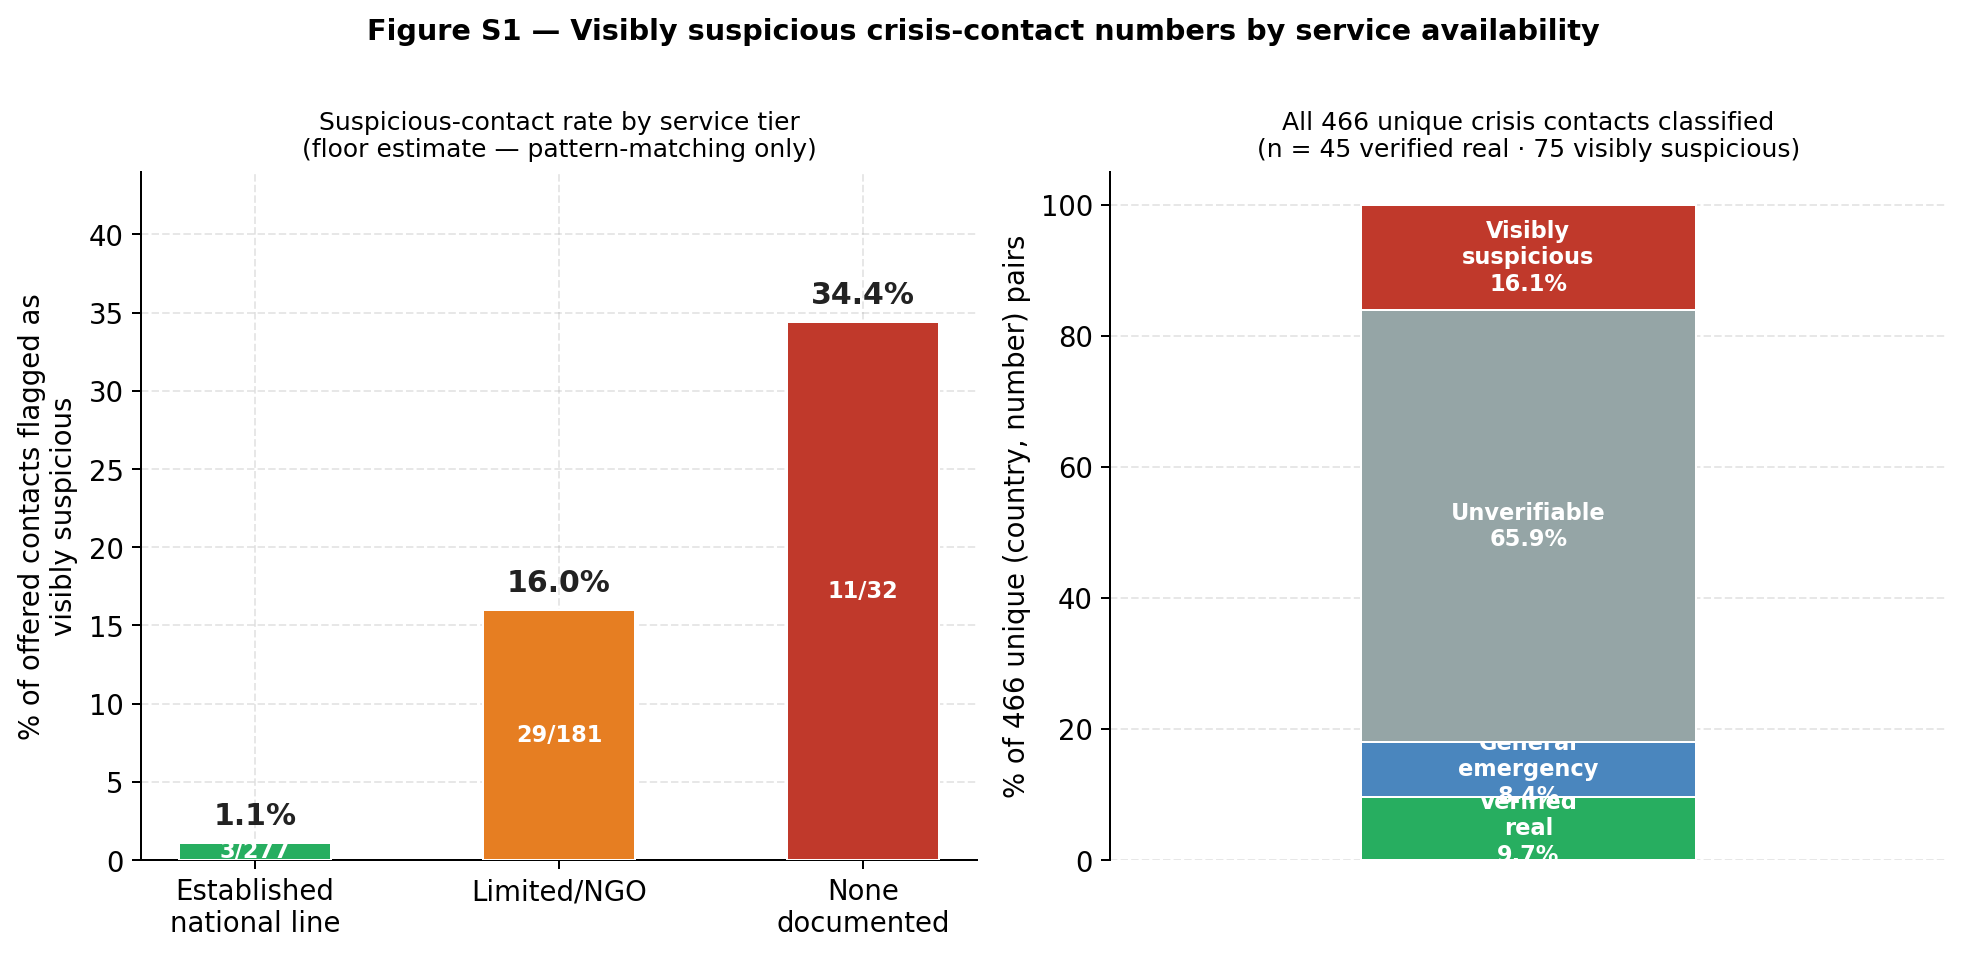
\includegraphics[width=0.75\textwidth]{Figure_S1_Fabrication.png}
\caption{Percentage of offered crisis-contact numbers displaying a visibly suspicious pattern, by documented service availability.}
\label{fig:s1}
\end{figure}

\section{Surface Versus Verified Localisation (H2 Sensitivity)}

\textbf{Question:} Does the H2 finding hold when the localisation contact component is restricted to numbers matched to documented services?

\textbf{Data:} Same 1,120 responses; \texttt{comp\_contact\_verified} constructed from the verification table. Of 490 responses containing a detected contact, 68 (13.9\%) contained a contact matched to a documented service; all 68 occurred in the established-national-line tier.

\textbf{Result:} Table~\ref{tab:surface_vs_verified}.

\begin{table}[H]
\centering
\caption{H2 under surface and verified localisation specifications (ref = None documented)}
\label{tab:surface_vs_verified}
\begin{tabular}{lcccc}
\toprule
Specification & \multicolumn{2}{c}{Limited/NGO} & \multicolumn{2}{c}{Established national line} \\
\cmidrule(lr){2-3} \cmidrule(lr){4-5}
 & Coef & $p$ & Coef & $p$ \\
\midrule
Surface (development-set $F_1 = 0.750$) & $+$0.251 & 0.012 & $+$0.353 & $<$0.001 \\
Verified (new) & $+$0.219 & 0.025 & $+$0.310 & 0.001 \\
\bottomrule
\end{tabular}
\end{table}

\textbf{Interpretation:} The direction is the same under both specifications and the verified-contact coefficients are slightly smaller. This is consistent with the direction of the surface-localisation association, but the verified measure has not itself been validated against human judgements and only 68 responses received verified-contact credit. It should therefore be treated as sensitivity evidence, not as a confirmed outcome.

\begin{figure}[H]
\centering
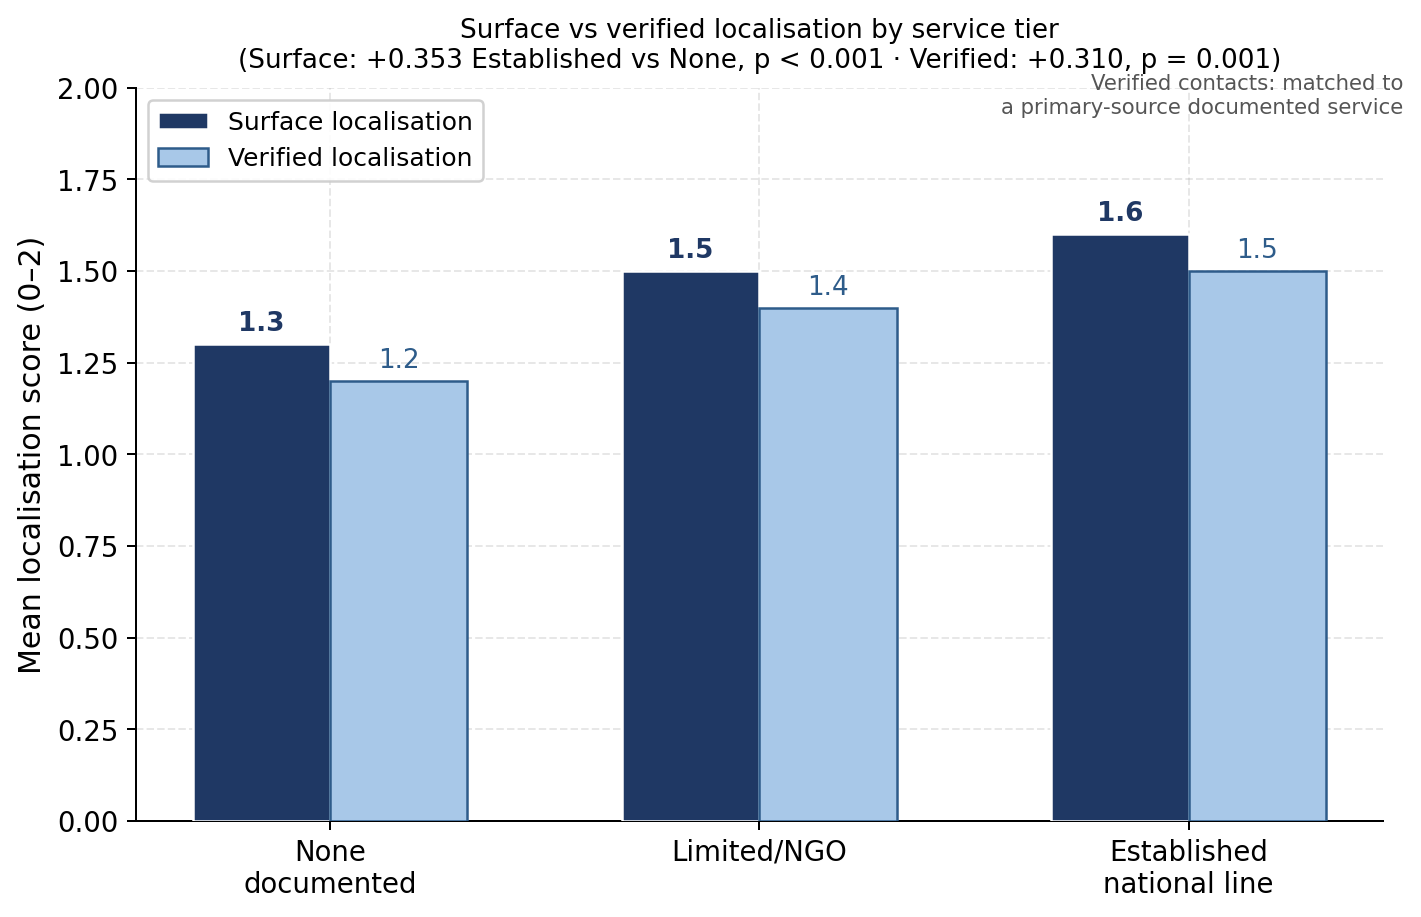
\includegraphics[width=0.92\textwidth]{Figure_H2_Surface_vs_Verified_Localisation.png}
\caption{Surface versus verified localisation by city, grouped by documented crisis-service availability. Surface (left) credits any contact present; verified (right) requires the contact to match a documented service.}
\label{fig:h2verif}
\end{figure}


\section{Sensitivity Analysis: Actionability Components}
\label{sec:sensitivity_components}

\textbf{Question:} Is the income gradient in actionability driven by all components equally, or concentrated in one?

\textbf{Method:} Each binary component of \texttt{actionability\_v2} tested separately against income category (Kruskal-Wallis). The composite is also refitted excluding the crisis-contact component.

\begin{table}[H]
\centering
\caption{Actionability component rates by income tier and Kruskal-Wallis significance. The income gradient is driven almost entirely by the crisis-contact component; all other components are non-significant or weakly significant.}
\label{tab:components}
\begin{tabular}{lccccc}
\toprule
Component & Low & Lower-Middle & Upper-Middle & High & KW sig. \\
\midrule
Crisis contact & 0.221 & 0.425 & 0.496 & 0.607 & *** \\
Professional referral & 0.221 & 0.321 & 0.321 & 0.282 & ns \\
Emergency escalation & 0.082 & 0.146 & 0.204 & 0.161 & * \\
Immediate action & 0.432 & 0.446 & 0.475 & 0.511 & ns \\
Named coping step & 0.596 & 0.636 & 0.586 & 0.571 & ns \\
\midrule
\textbf{actionability\_v2 (sum)} & 1.554 & 1.939 & 2.029 & 2.132 & *** \\
\textbf{Excluding crisis contact} & 1.332 & 1.514 & 1.532 & 1.525 & ns \\
\bottomrule
\end{tabular}
\end{table}

\textbf{Interpretation (corrected):} The income gradient in \texttt{actionability\_v2} is driven almost entirely by the crisis-contact component. When crisis contact is excluded, the gradient disappears (KW $p = 0.25$). This clarifies the mechanism: income differences in actionability reflect differences in crisis-contact inclusion, not differences in professional referral quality, coping guidance, or urgency language.

\section{Joint Income and Service-Availability Model}
\label{sec:joint_model}

\textbf{Question:} After controlling for documented crisis-service availability, does the income gradient remain?

\textbf{Method:} Linear mixed-effects model with both income category and service-availability tier as predictors simultaneously, plus model identity, scenario, and city random intercept.

\begin{table}[H]
\centering
\caption{Joint model: actionability\_v2 $\sim$ income + service availability + model + scenario + (1$\mid$city). When both predictors are included, income becomes non-significant while service availability remains significant.}
\label{tab:joint}
\begin{tabular}{lcccc}
\toprule
Predictor & Coef & 95\% CI & $p$ & Sig. \\
\midrule
High vs Low (income) & $+$0.233 & [$-$0.109, $+$0.575] & 0.183 & ns \\
Upper-Middle vs Low & $+$0.151 & [$-$0.204, $+$0.507] & 0.405 & ns \\
Lower-Middle vs Low & $+$0.062 & [$-$0.294, $+$0.418] & 0.733 & ns \\
\textbf{Established vs None (service)} & $\mathbf{+0.446}$ & \textbf{[$+$0.099, $+$0.794]} & \textbf{0.012} & \textbf{*} \\
\textbf{Limited/NGO vs None} & $\mathbf{+0.391}$ & \textbf{[$+$0.002, $+$0.779]} & \textbf{0.049} & \textbf{*} \\
\bottomrule
\end{tabular}
\end{table}

\textbf{Interpretation:} Income does not independently predict actionability once service availability is controlled. The mechanism appears to be that higher-income countries tend to have more documented crisis services, and it is the presence of those services --- not income per se --- that drives the actionability difference. This is a more conservative and more defensible interpretation than claiming an income effect directly.

\textbf{Limitation:} Income and service availability are partially collinear in this 20-city sample (higher-income countries tend to have established national lines). With only 20 cities, the joint model has limited power to separate the two predictors. The finding is consistent with a service-mediation mechanism but does not establish it definitively.

\textbf{Decision:} The H1 conclusion is revised. Rather than claiming ``actionability increases with income'', the more defensible claim is: ``crisis-contact inclusion increases with the availability of documented national crisis services, and income correlates with service availability.'' The original H1 result (+0.614) remains valid as a descriptive finding; the joint model provides the explanatory context.

\section{Summary of Results}

Table~\ref{tab:results_summary} provides a single-view summary of all four findings.

\begin{table}[H]
\centering
\caption{Summary of all results}
\label{tab:results_summary}
\begin{tabular}{llccc}
\toprule
Finding & Outcome / measure & Effect & $p$ & Validated $F_1$ \\
\midrule
H1 (RQ1) & Actionability, High vs Low income & $+$0.614 & $<$0.001 & 0.744 \\
H2 (RQ2) & Localisation, Established vs None & $+$0.353 & $<$0.001 & 0.750 \\
H3 (RQ3) & Religious framing, EUR vs AFR & OR = 0.015 & 0.003 & 0.889 \\
S1 (unplanned) & Visibly suspicious contacts, None documented & 34.4\% & --- & floor est. \\
\bottomrule
\end{tabular}
\end{table}
